\documentclass[border=0.2cm, convert={density=600}]{standalone}
 
% Required packages and libraries
\usepackage{tikz}
\usetikzlibrary{shapes, positioning, arrows.meta, calc}

% custom styles
\tikzset{
  parser/.style={
    rectangle,
    rounded corners,
    draw=black, very thick,
    minimum height=2em,
    inner sep=2pt,
    text centered,
    rectangle split,
    rectangle split draw splits=false,
    rectangle split parts=2,
    draw=black
  },
  arrow/.style={
    draw=black,
    thick,
    ->,
    >=stealth
  }
}

% custom dot symbol (bigger than \cdot but smaller than \bullet)
\makeatletter
\newcommand*\dotp{\mathpalette\dotp@{.5}}
\newcommand*\dotp@[2]{\mathbin{\vcenter{\hbox{\scalebox{#2}{$\m@th#1\bullet$}}}}}
\makeatother
 
\begin{document}
 
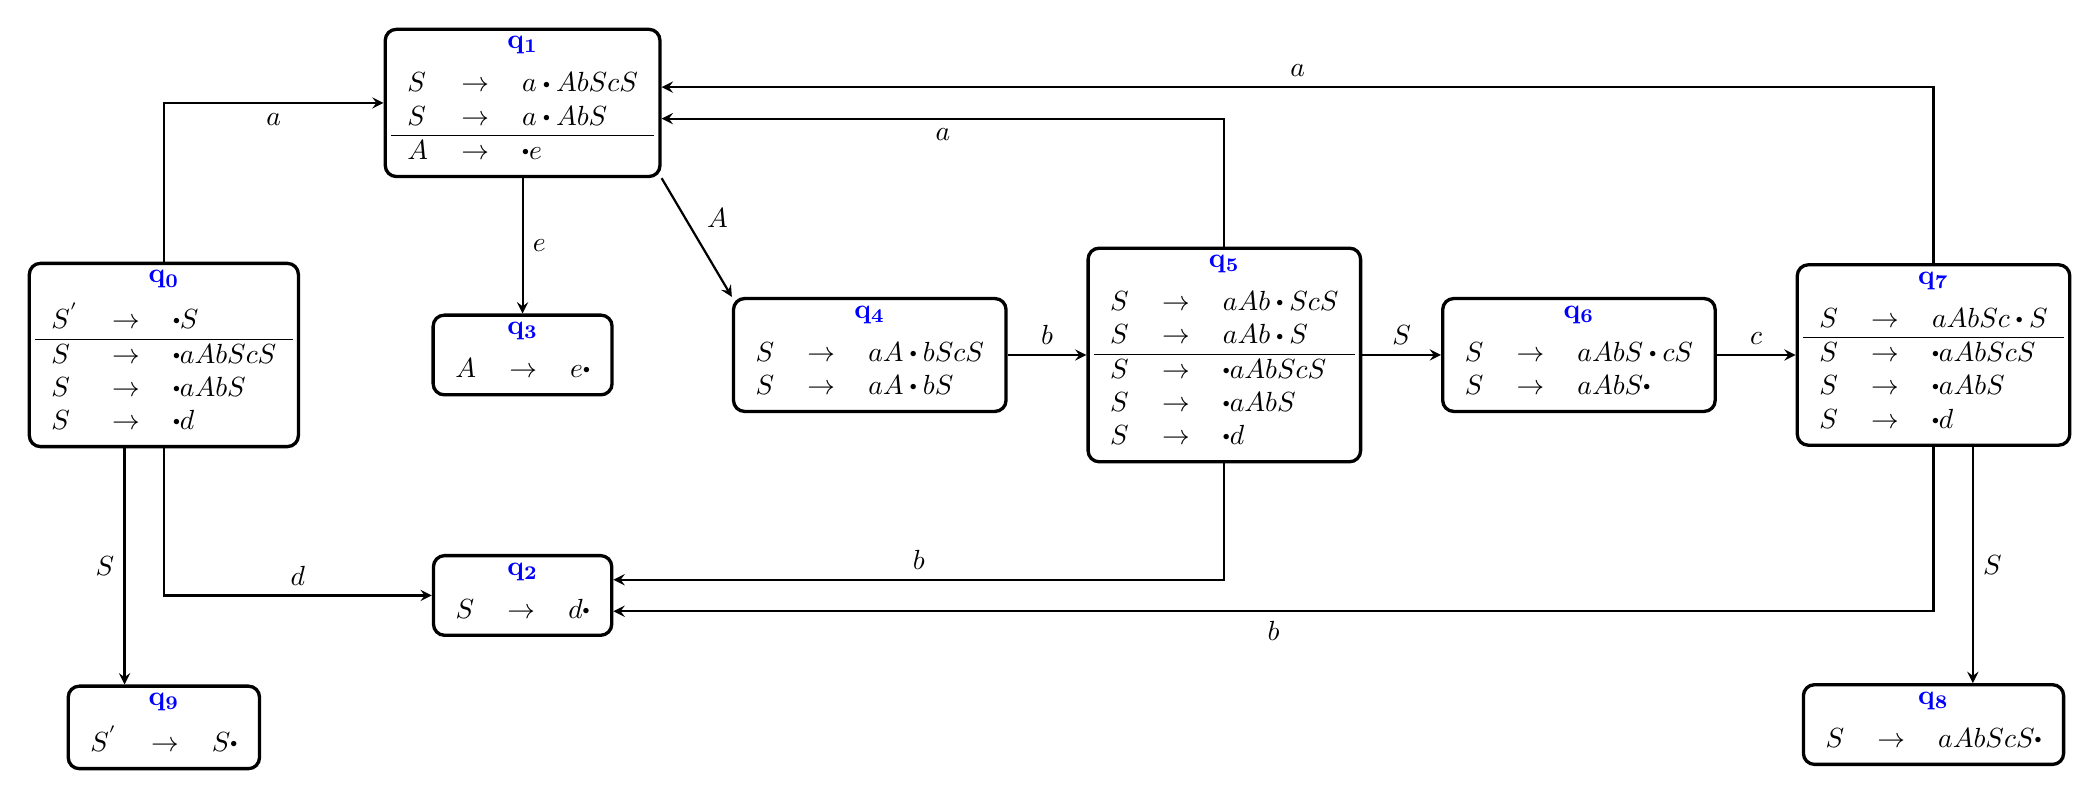
\begin{tikzpicture}
% LR(0)/SLR(1) Parser
% Grammar:
%   (0) S' → S
%	(1) S  → a A b S c S
%	(2) S  → a A b S
%	(3) S  → d
%	(4) A  → e

% nodes
\node[parser] (q0)
{ $\mathbf{\color{blue} q_{0}}$
  \nodepart{second}
  \begin{tabular}{lll}
      $S^{'}$ & $\rightarrow$ & $\dotp S$ \\
      \hline
      $S$     & $\rightarrow$ & $\dotp aAbScS$ \\
      $S$     & $\rightarrow$ & $\dotp aAbS$ \\
      $S$     & $\rightarrow$ & $\dotp d$ \\
  \end{tabular}
};

\node[parser, above right = 1.5cm of q0.north east, anchor=south west] (q1)
{ $\mathbf{\color{blue} q_{1}}$
  \nodepart{second}
  \begin{tabular}{lll}
      $S$ & $\rightarrow$ & $a \dotp AbScS$ \\
      $S$ & $\rightarrow$ & $a \dotp AbS$ \\
      \hline
      $A$ & $\rightarrow$ & $\dotp e$ \\
  \end{tabular}
};

\node[parser] (q3) at (q0.east -| q1.south)
{ $\mathbf{\color{blue} q_{3}}$
  \nodepart{second}
  \begin{tabular}{lll}
      $A$ & $\rightarrow$ & $e \dotp$\\
  \end{tabular}
};

\node[parser, below = 2cm of q3.south, anchor=north] (q2)
{ $\mathbf{\color{blue} q_{2}}$
  \nodepart{second}
  \begin{tabular}{lll}
      $S$ & $\rightarrow$ & $d \dotp$\\
  \end{tabular}
};

\node[parser, right = 1.5cm of q3.east, anchor=west] (q4)
{ $\mathbf{\color{blue} q_{4}}$
  \nodepart{second}
  \begin{tabular}{lll}
      $S$ & $\rightarrow$ & $aA \dotp bScS$\\
      $S$ & $\rightarrow$ & $aA \dotp bS$\\
  \end{tabular}
};

\node[parser, right = 1cm of q4.east, anchor=west] (q5)
{ $\mathbf{\color{blue} q_{5}}$
  \nodepart{second}
  \begin{tabular}{lll}
      $S$ & $\rightarrow$ & $aAb \dotp ScS$\\
      $S$ & $\rightarrow$ & $aAb \dotp S$\\
      \hline
      $S$ & $\rightarrow$ & $\dotp aAbScS$\\
      $S$ & $\rightarrow$ & $\dotp aAbS$\\
      $S$ & $\rightarrow$ & $\dotp d$\\
  \end{tabular}
};

\node[parser, right = 1cm of q5.east, anchor=west] (q6)
{ $\mathbf{\color{blue} q_{6}}$
  \nodepart{second}
  \begin{tabular}{lll}
      $S$ & $\rightarrow$ & $aAbS \dotp cS$\\
      $S$ & $\rightarrow$ & $aAbS \dotp $\\
  \end{tabular}
};

\node[parser, right = 1cm of q6.east, anchor=west] (q7)
{ $\mathbf{\color{blue} q_{7}}$
  \nodepart{second}
  \begin{tabular}{lll}
      $S$ & $\rightarrow$ & $aAbSc \dotp S$\\
      \hline
      $S$ & $\rightarrow$ & $\dotp aAbScS$\\
      $S$ & $\rightarrow$ & $\dotp aAbS$\\
      $S$ & $\rightarrow$ & $\dotp d$\\
  \end{tabular}
};

\node[parser, below = 3cm of q7.south, anchor=north] (q8)
{ $\mathbf{\color{blue} q_{8}}$
  \nodepart{second}
  \begin{tabular}{lll}
      $S$ & $\rightarrow$ & $aAbScS\dotp$\\
  \end{tabular}
};

\node[parser, below = 3cm of q0.south, anchor=north] (q9)
{ $\mathbf{\color{blue} q_{9}}$
  \nodepart{second}
  \begin{tabular}{lll}
      $S^{'}$ & $\rightarrow$ & $S\dotp$\\
  \end{tabular}
};

% edges

%% q0
\draw [arrow] (q0.north) -- (q0.north |- q1.west) -- node[anchor=north]{$a$} (q1.west);
\draw [arrow] (q0.south) -- (q0.south |- q2.west) -- node[anchor=south]{$d$} (q2.west);
\draw [arrow, transform canvas={xshift=-5mm}] (q0.south) -- node[anchor=east]{$S$} (q9.north);

%% q1
\draw [arrow] (q1.south) -- node[anchor=west]{$e$} (q3.north);
\draw [arrow] (q1.south east) -- node[anchor=south west]{$A$} (q4.north west);

%% q4
\draw [arrow] (q4.east) -- node[anchor=south]{$b$} (q5.west);

%% q5
\draw [arrow] (q5.east) -- node[anchor=south]{$S$} (q6.west);
\coordinate[below=2mm of q1.east] (h51);
\draw [arrow] (q5.north) -- (q5.north |- h51)-- node[anchor=north]{$a$} (h51);
\coordinate[above=2mm of q2.east] (h52);
\draw [arrow] (q5.south) -- (q5.south |- h52)-- node[anchor=south]{$b$} (h52);

%% q6
\draw [arrow] (q6.east) -- node[anchor=south]{$c$} (q7.west);

%% q7
\draw [arrow, transform canvas={xshift=5mm}] (q7.south) -- node[anchor=west]{$S$} (q8.north);
\coordinate[above=2mm of q1.east] (h71);
\draw [arrow] (q7.north) -- (q7.north |- h71)-- node[anchor=south]{$a$} (h71);
\coordinate[below=2mm of q2.east] (h72);
\draw [arrow] (q7.south) -- (q7.south |- h72)-- node[anchor=north]{$b$} (h72);

\end{tikzpicture}
 
\end{document}
